% #!$HOME/.asdf/install/python/$PYTHON_MAJOR_MINOR/bin/python$PYTHON_MAJOR

\documentclass[12pt]{article}

\usepackage{sbc-template}

\usepackage{graphicx,url}
\usepackage{float}

%\usepackage[brazil]{babel}   
\usepackage[utf8]{inputenc}  

     
\sloppy

\title{Unikernel}

\author{Eduardo Henrique Mendel\inst{1}, Gabriel Porto dos Santos\inst{1}, Guilherme Gonçalves\inst{1}}


\address{
  Escola Politécnina- Universidade do Vale do Rio dos Sinos\\
  93022-750 -- São Leopoldo -- RS -- Brazil
  \email{\{gaporto\}@edu.unisinos.br}
} % Colocar ", [usuário]" entre os "{}" no campo de e-mail, ao lado do meu \{gaporto}\

\begin{document} 

\maketitle
% ! TODO Remove - (! \label WIP)
% O Lorem é para ter noção de espaço (máximo) para garantir
% o respeito de número máximo de páginas.
\begin{abstract}
Lorem ipsum dolor sit amet, consectetur adipiscing elit. Integer consequat sed est quis pellentesque. Curabitur vitae mi porttitor nunc porta lacinia tempus eget metus. Nam eu nunc eu mi blandit interdum. Quisque tempor eget velit sit amet feugiat. Phasellus elementum feugiat risus, id rutrum augue scelerisque in. Praesent aliquet varius libero sit amet lacinia. Donec consectetur non nisi et tincidunt. Nullam a est et nisi fringilla volutpat. Integer mauris lorem, congue id mattis eu, ultricies sit amet ligula. Suspendisse potenti. Ut volutpat, dui eu vestibulum ornare, mauris sem sollicitudin quam, eu tincidunt felis nunc sagittis purus. Integer eleifend justo nec sagittis pulvinar. Quisque mollis id justo sit amet interdum. Etiam a turpis varius nunc pharetra. 
\end{abstract}
% ! TODO Remove - (! \label WIP)
% O Lorem é para ter noção de espaço (máximo) para garantir
% o respeito de número máximo de páginas.     
\begin{resumo} 
Lorem ipsum dolor sit amet, consectetur adipiscing elit. Integer consequat sed est quis pellentesque. Curabitur vitae mi porttitor nunc porta lacinia tempus eget metus. Nam eu nunc eu mi blandit interdum. Quisque tempor eget velit sit amet feugiat. Phasellus elementum feugiat risus, id rutrum augue scelerisque in. Praesent aliquet varius libero sit amet lacinia. Donec consectetur non nisi et tincidunt. Nullam a est et nisi fringilla volutpat. Integer mauris lorem, congue id mattis eu, ultricies sit amet ligula. Suspendisse potenti. Ut volutpat, dui eu vestibulum ornare, mauris sem sollicitudin quam, eu tincidunt felis nunc sagittis purus. Integer eleifend justo nec sagittis pulvinar. Quisque mollis id justo sit amet interdum. Etiam a turpis varius nunc pharetra.
\end{resumo}

\section{Introdução}

Em relação aos Sistemas Operacionais modernos, a virtualização, contemporaneamente, mostra-se como um tópico imprescindível para o desenvolvimento de aplicações dada a ênfase na conteinerização e modularização de aspectos de infraestrutura em realidades como a \textit{IoT}, por exemplo. Devido a tópicos como este, há a utilização de funcionalidades destes por meio de \textit{Cloud} ou módulos embarcados a fim de aumentar suas possibilidades de um dado sistema. Todavia, esta abordagem possui um problema intrínseco: a complexidade do Kernel do sistema que a mantém. No caso do Linux, seu Kernel é relativamente flexível, mas em determinados contextos onde é empregado pode vir a se tornar um problema quanto a performance e portabilidade.

A fim de sobrepor situações não benéficas relacionados a este problema estrutural, emprega-se o \textit{Unikernel}. Este é definido por ser uma abordagem por intermédio de bibliotecas específicas de componentes do sistema operacional que provém as mesmas a aplicação requerente da funcionalidade \cite{raza:196}, tornando-se ordens de grandeza mais eficiente quando comparado a uma virtualização completa e literal do sistema operacional utilizado.

O conceito fundamenta-se, basicamente, da utilização do sistema operacional semelhante ao uso de uma biblioteca - como por exemplo o \textit{mirageOS}. Vários módulos são carregados por intermédio de determinadas camadas de abstração que, dependendo de seu objetivo, são carregadas de forma mais eficiente no ambiente que a requer. Deste modo, esta "granulação" da arquitetura de um sistema operacional impede que o mesmo trate processos de modo a utilizar ferramentas para o tratamento multitarefa dos mesmos. O que ocorre é a compilação do mesmo a fim de proporcionar sua execução como processo único, tendo seu funcionamento e organização em geral semelhante a de um microsserviço \cite{fraga:120}.

\section{Arquitetura}

Em seu cerne, Unikernels são estruturados para funcionarem baseados na necessidade do sistema, isto é, o mesmo carateriza-se por ser orientado a serviço (\textit{service-based}). Desta forma, sua organização e arquitetura fundamentam-se em melhor atender a estas necessidades baseadas no módulos requeridos, utilizando uma abordagem cirúrgica e objetiva, quando comparado ao modelo de virtualização de um sistema operacional ou outras abordagens, como visto na figura ~\ref{fig:fig1}.

\begin{figure}[H]
\centering
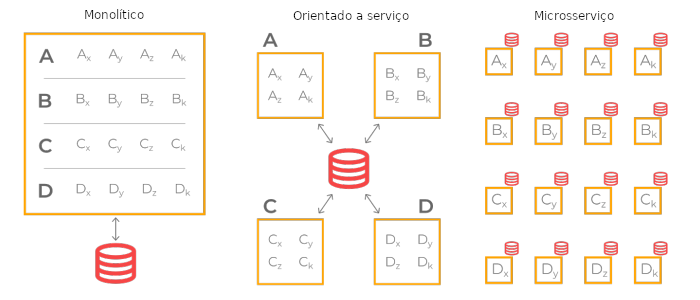
\includegraphics[width=.8\textwidth]{fig1.png}
\caption{Comparação das abordagens com um banco de dados de exemplo. Fonte: Adaptado de \cite{fraga:120}}
\label{fig:fig1}
\end{figure}


\subsection{Estrutura}

 Na mesma figura, utilizando como comparação a utilização de um banco de dados, exemplifica-se que a "granulação", diferente de uma alternativa mais monolítica de um sistema operacional ou orientada a serviço, módulos de Unikernel são um "universo próprio". Ou seja, não há dependências que não as unicamente necessária para sua funcionalidade e por consequência \textit{overheads} geradas pela utilização de certos recursos. 
 
 Esta mitigação de recursos aos moldes de microsserviços é extremamente eficiente quando aplicada a aplicações de \textit{IoT}, sendo estes - principalmente quando vinculado às aplicações \textit{Cloud} - fundamentalmente desenvolvidos para ser altamente escaláveis e distribuídos, tendo como este o principal fator da utilização em determinados contextos \cite{fraga:120}.
 
 Partindo deste tópico, considerando que estes módulos são ordens de grandeza menores que o modelo de um sistema inteiro, existem uma série de fatores que se destacam em sua construção, sendo um dos mais importantes o aspecto relacionado à segurança do mesmo. Tal conceito é abrangido e assegurado principalmente na não dependência de terceiros não requeridos, mas, mais fundamentalmente, pela imutabilidade do módulo. 
 
 \subsection{Organização}
 
 Define-se esta imutabilidade como, ao criar o módulo, este apenas conterá um singelo espaço de endereçamento contendo tudo aquilo que precisará para seu funcionamento pleno. Graças a esta abordagem contida, diferentemente de sistemas operacionais (como os *NIX/BSD) não há existência de modos de execução, ou seja, não há \textit{kernel-mode} e \textit{user-mode}, como o demostrado pelo comparativo da figura ~\ref{fig:fig2}.

\begin{figure}[H]
\centering
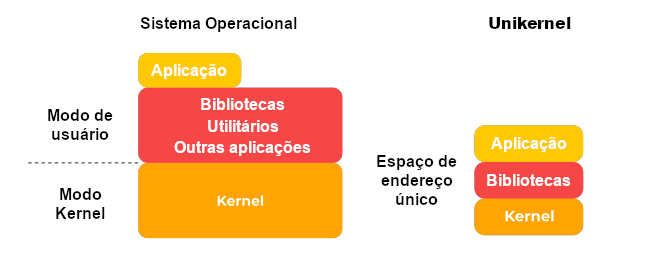
\includegraphics[width=.8\textwidth]{fig2.png}
\caption{Comparação de um sistema operacional e um módulo Unikernel. Fonte: Adaptado de \cite{fraga:120}}
\label{fig:fig2}
\end{figure}

 Esta mudança trás consigo, principalmente, a não necessidade de troca de contexto para acesso de determinados recursos - e, portanto, não tras consigo seus \textit{overheads}, sendo este um outro atrativo a favor de sua utilização. A princípio, tal alteração pode parecer insegura, porém, mostra-se eficiente e até mesmo mais inabalável quanto a este tópico em relação às abordagens que fazem uso de sistemas operacionais "inteiros".
 
 O ocorrido é que, dada sua granularidade e seu contexto extremamente específico, mesmo que haja algum problema, este não é capaz de alterar o sistema que utilizará estes módulos em sua totalidade. No caso de, por exemplo, uma invasão, o atacante terá acesso apenas ao módulo em questão, sendo incapaz de interferir em outros processos - a menos que o mesmo seja capaz de interagir diretamente com o \textit{Hypervisor} \cite{fraga:120}. 
 
 \subsection{Hypervisor}
 
 Unikernels, assim como qualquer Máquina Virtual, necessitam obrigatoriamente de um meio de acesso ao hardware para que funcionem. Nesta situação, utiliza-se um mecanismo para servir de barramento entre camadas lógicas e físicas, o mesmo é conhecido como \textit{Hypervisor}.
 
 Quanto a sua aplicação aos módulos do Unikernel, sua funcionalidade difere quando comparada a um simples Máquina Virtual. O mesmo além de barramento, serve como agregador de cada módulo, possibilitando, por exemplo interações dentre os módulos tal qual programas que seguem filosofia UNIX de software. Todavia, em contraponto, \textit{Hypervisors} para Unikernels não \textbf{(WIP terminar de citar as diferenças do Hypervisor utilizado em Unikerls (usando a foto de ref da pg 21 do \cite{fraga:120}. Seguido de citar virtualização [integrar o doc adaptando] e por último falar de desempenho). Se necessário, dar uma resumida para não passar as cinco pgs, mas acho que foi resumido e dará certo} % ! TODO Continuar amanhã (09/06) | Remove - (! \label WIP)

\bibliographystyle{sbc}
\bibliography{sbc-template}

\end{document}
